\documentclass{article}

% Idioma
\usepackage[spanish]{babel}

% márgenes y formato
\usepackage[a4paper,top=2cm,bottom=2cm,left=3cm,right=3cm,marginparwidth=1.75cm]{geometry}
\usepackage{parskip}

% Otros paquetes importantes
\usepackage{amsmath}
\usepackage{amssymb}
\usepackage{graphicx}
\usepackage[colorlinks=true, linkcolor=black, urlcolor=blue]{hyperref}

% PARA APUNTES: darkmode
% \usepackage{darkmode}
% \enabledarkmode

% Titulo y autor
\title{Métodos de Runge-Kutta}
\author{Álvaro Hernández Riquelme}
\date{\today}

\begin{document}

%%%%%%%%%%%%%%%%%%%%%%%%%%%%%%%%%%

\maketitle
\tableofcontents
\newpage

\section{Introducción}

Se considera la siguiente ecuación diferencial ordinaria (EDO), que es la misma del ejercicio anterior:
$$ y'(x) = 4x + y(x)^2 $$
junto con la condición inicial:
$$ y(0) = 1 $$
El objetivo es aproximar la solución en el punto final $b = 0.04$.

\section{Primeros ejercicios}
\subsection{Completar el tablero para el orden y etapas proporcionadas.}

Se nos pide encontrar el único método Runge-Kutta explícito de $s=3$ etapas y orden $n=3$ que tiene los coeficientes $c_2 = \frac{2}{5}$ y $c_3=1$. El tablero a completar es:
$$
\begin{array}{c|ccc}
c_1 & 0 & 0 & 0 \\
c_2 & a_{21} & 0 & 0 \\
c_3 & a_{31} & a_{32} & 0 \\
\hline
& b_1 & b_2 & b_3
\end{array}
=
\begin{array}{c|ccc}
c_1 & 0 & 0 & 0 \\
2/5 & a_{21} & 0 & 0 \\
1 & a_{31} & a_{32} & 0 \\
\hline
& b_1 & b_2 & b_3
\end{array}
$$
Para determinar los coeficientes desconocidos, utilizaremos las condiciones de simplificación y las ecuaciones de orden para métodos Runge-Kutta, como se describe en el pdf de teoría.

Lo primero será aplicar las condiciones de simplificación. La condición $c_j = \sum_{k=1}^{j-1} a_{j,k}$ se asume como cierta.

\begin{itemize}
    \item Para $j=1$: $c_1 = 0$ (la suma es vacía).
    \item Para $j=2$: $c_2 = a_{21}$. Dado que $c_2 = 2/5$, tenemos que $\boldsymbol{a_{21} = 2/5}$.
    \item Para $j=3$: $c_3 = a_{31} + a_{32}$. Dado que $c_3 = 1$, obtenemos la ecuación $\boldsymbol{a_{31} + a_{32} = 1}$.
\end{itemize}

Las ecuaciones de orden nos proporcionan un sistema de ecuaciones para los coeficientes $b_j$ y $a_{j,k}$.

\textbf{Orden 1:} $\sum_{j=1}^{3} b_j = 1 \implies b_1 + b_2 + b_3 = 1$

\textbf{Orden 2:} $\sum_{j=1}^{3} b_j c_j = \frac{1}{2} \implies b_1(0) + b_2(\frac{2}{5}) + b_3(1) = \frac{1}{2} \implies \frac{2}{5}b_2 + b_3 = \frac{1}{2}$

\textbf{Orden 3:} Se deben cumplir dos condiciones:
\begin{enumerate}
    \item $\sum_{j=1}^{3} b_j c_j^2 = \frac{1}{3} \implies b_1(0)^2 + b_2(\frac{2}{5})^2 + b_3(1)^2 = \frac{1}{3} \implies \frac{4}{25}b_2 + b_3 = \frac{1}{3}$
    \item $\sum_{j,k} b_j a_{j,k} c_k = \frac{1}{6}$. Para un método explícito de 3 etapas, se expande a $b_2 a_{21} c_1 + b_3(a_{31}c_1 + a_{32}c_2) = \frac{1}{6}$. Como $c_1=0$, la ecuación se simplifica a: $b_3 a_{32} c_2 = \frac{1}{6} \implies b_3 a_{32} (\frac{2}{5}) = \frac{1}{6}$
\end{enumerate}

Finalmente resolvemos el sistema de ecuaciones. Primero resolvemos para $b_2$ y $b_3$.

\begin{align*}
    \frac{2}{5}b_2 + b_3 &= \frac{1}{2} \\
    \frac{4}{25}b_2 + b_3 &= \frac{1}{3}
\end{align*}
Restando la segunda ecuación de la primera:
$$ \left(\frac{2}{5} - \frac{4}{25}\right)b_2 = \frac{1}{2} - \frac{1}{3} \implies \left(\frac{10-4}{25}\right)b_2 = \frac{3-2}{6} \implies \frac{6}{25}b_2 = \frac{1}{6} \implies \boldsymbol{b_2 = \frac{25}{36}} $$
Sustituyendo $b_2$ en la primera ecuación:
$$ b_3 = \frac{1}{2} - \frac{2}{5}b_2 = \frac{1}{2} - \frac{2}{5}\left(\frac{25}{36}\right) = \frac{1}{2} - \frac{5}{18} = \frac{9-5}{18} = \frac{4}{18} \implies \boldsymbol{b_3 = \frac{2}{9}} $$
Ahora, con la condición de orden 1, encontramos $b_1$:
$$ b_1 = 1 - b_2 - b_3 = 1 - \frac{25}{36} - \frac{2}{9} = \frac{36 - 25 - 8}{36} = \frac{3}{36} \implies \boldsymbol{b_1 = \frac{1}{12}} $$
Finalmente, usamos la ecuación de orden 3.2 y la de simplificación para $c_3$:
$$ b_3 a_{32} \left(\frac{2}{5}\right) = \frac{1}{6} \implies \frac{2}{9} a_{32} \frac{2}{5} = \frac{1}{6} \implies a_{32} = \frac{1}{6} \cdot \frac{45}{4} \implies \boldsymbol{a_{32} = \frac{15}{8}} $$
$$ a_{31} = 1 - a_{32} = 1 - \frac{15}{8} \implies \boldsymbol{a_{31} = -\frac{7}{8}} $$

El tablero completo para el método de orden 3 es:

$$
\begin{array}{c|ccc}
0 & 0 & 0 & 0 \\
2/5 & 2/5 & 0 & 0 \\
1 & -7/8 & 15/8 & 0 \\
\hline
& 1/12 & 25/36 & 2/9
\end{array}
$$

\subsection{Aplicar N=1 paso (h=0.04)}

Usamos el método anterior para dar un único paso de longitud $h=0.04$.
La función es $f(x,y) = 4x + y^2$. Partimos de $(x_0, y_0) = (0, 1)$.

Calculamos las etapas $K_j=f(x_0+c_j h, y_0+h\sum a_{j,k}K_k)$:
\begin{align*}
    K_1 &= f(x_0, y_0) = f(0, 1) = 4(0) + 1^2 = \boxed{1} \\ \\
    K_2 &= f(x_0 + c_2 h, y_0 + h a_{21} K_1) \\
        &= f(0 + \frac{2}{5}(0.04), 1 + 0.04 \cdot \frac{2}{5} \cdot 1) \\
        &= f(0.016, 1.016) = 4(0.016) + (1.016)^2 = 0.064 + 1.032256 = \boxed{1.096256} \\ \\
    K_3 &= f(x_0 + c_3 h, y_0 + h(a_{31}K_1 + a_{32}K_2)) \\
        &= f(0.04, 1 + 0.04(-\frac{7}{8} \cdot 1 + \frac{15}{8} \cdot 1.096256)) \\
        &= f(0.04, 1 + 0.04(1.18048)) \\
        &= f(0.04, 1.0472192) = \boxed{1.25666805284864}
\end{align*}
Finalmente, calculamos la aproximación $y_1$:
\begin{align*}
    y_1 &= y_0 + h(b_1 K_1 + b_2 K_2 + b_3 K_3) \\
        &= 1 + 0.04 \left( \frac{1}{12}(1) + \frac{25}{36}(1.096256) + \frac{2}{9}(1.25666805284864) \right) \\
        &= 1 + 0.04\,(1.12388178952192) \\
        &\approx 1.0449552715808768
\end{align*}

\subsection{Aplicar N=2 pasos (h=0.02)}

Ahora damos dos pasos de longitud \(h=0.02\) para llegar al mismo punto final \(b=0.04\).

\subsection*{Paso 1: \(x_0 = 0 \to x_1 = 0.02\)}
Las condiciones iniciales son \((x_0, y_0) = (0, 1)\) y \(h=0.02\).
\begin{align*}
    K_1 &= f(0, 1) = \boxed{1} \\
    K_2 &= f(0 + \frac{2}{5}(0.02), 1 + 0.02 \cdot \frac{2}{5} \cdot 1) = f(0.008, 1.008) = \boxed{1.048064} \\
    K_3 &= f(0.02, 1 + 0.02(-\frac{7}{8} \cdot 1 + \frac{15}{8} \cdot 1.048064)) = f(0.02, 1.0218024) = \boxed{1.1240801446457602}
\end{align*}
La aproximación en \(x_1=0.02\) es:
\begin{align*}
    y_1 &= 1 + 0.02 \left( \frac{1}{12}(1) + \frac{25}{36}(1.048064) + \frac{2}{9}(1.1240801446457602) \right) \\
        &= \boxed{1.0212190228650924}
\end{align*}

\subsection*{Paso 2: \(x_1 = 0.02 \to x_2 = 0.04\)}

Las nuevas condiciones iniciales son \((x_1, y_1) = (0.02, 1.0212190228650924)\) y \(h=0.02\).
\begin{align*}
    K_1 &= f(0.02, 1.0212190228650924) = \boxed{1.122888292661534} \\
    K_2 &= f(0.028, 1.0212190228650924 + 0.02 \cdot \frac{2}{5} \cdot K_1) = f(0.028, 1.0302021292063845) = \boxed{1.1733164270213683} \\
    K_3 &= f(0.04, 1.0212190228650924 + 0.02(-\frac{7}{8} \cdot K_1 + \frac{15}{8} \cdot K_2)) = f(0.04, 1.0455678437568168) = \boxed{1.2532121158982792}
\end{align*}
La aproximación final en \(x_2=0.04\) es:
\begin{align*}
    y_2 &= 1.0212190228650924 + 0.02 \left( \frac{1}{12}(K_1) + \frac{25}{36}(K_2) + \frac{2}{9}(K_3) \right) \\
        &= \boxed{1.044956396465484}
\end{align*}


\subsection{Aplicar N=4 pasos (h=0.01)}
Realizar cuatro pasos a mano es muy tedioso. El procedimiento es lo mismo que los ejercicios anteriores, llamando a la función de MAXIMA con variables definidas anteriormente, el resultado sale tal que:

\begin{figure}[h]
    \centering
    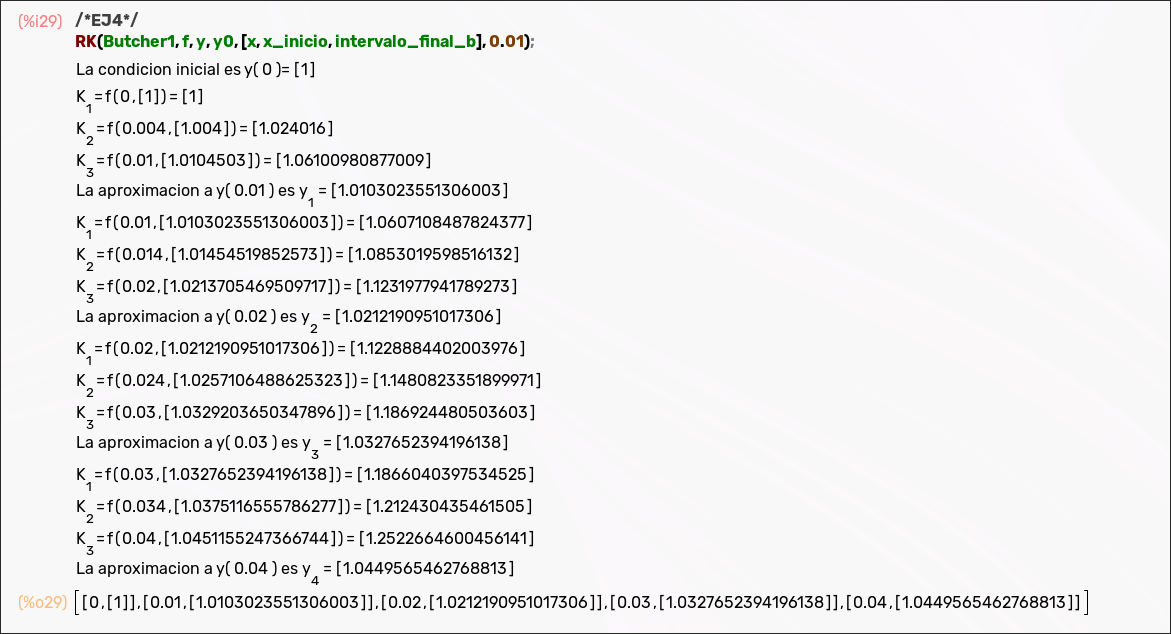
\includegraphics[width=0.8\textwidth]{src/ej4.png}
    \caption{Resultados del ejercicio 4}
    \label{fig:ejercicio4}
\end{figure}


\subsection{Comparación con el método de Taylor}


Al comparar el resultado obtenido, siendo el de este ejercicio $y(0.04) \approx 1.04495654...$ con el del ejercicio anterior $1,044949333$ apreciamos una similitud. La ventaja de los métodos Runge-Kutta es que alcanzan un orden de precisión alto sin necesidad de calcular las derivadas sucesivas de la función $f(x,y)$ y con una complejidad menor que el método de Taylor.


\section{Ejercicios finales}
\subsection{Encontrar los coeficientes $\hat{b_1}$, $\hat{b_2}$, $\hat{b_3}$}

Para que el método tenga orden 2, los coeficientes deben satisfacer las condiciones:

$$
\sum_{i=1}^{3} \hat{b}_{i} = 1 \quad \text{y} \quad \sum_{i=1}^{3} \hat{b}_{i} c_{i} = \frac{1}{2}
$$

Con los valores del tablero $c_1=0$, $c_2=2/5$, $c_3=11/10$ y el parámetro $\hat{b}_3 = \lambda$, como se aconseja en en el enunciado, tenemos:

$$
\begin{cases}
\hat{b}_{1} + \hat{b}_{2} + \lambda = 1 \\
\hat{b}_{1} \cdot 0 + \hat{b}_{2} \cdot \frac{2}{5} + \lambda \cdot \frac{11}{10} = \frac{1}{2}
\end{cases}
$$
De la segunda ecuación, despejamos $\hat{b}_2$:
$$
\frac{2}{5}\hat{b}_{2} = \frac{1}{2} - \frac{11}{10}\lambda \implies \hat{b}_{2} = \frac{5}{2} \left( \frac{5 - 11\lambda}{10} \right) = \frac{5 - 11\lambda}{4}
$$
Sustituimos $\hat{b}_2$ en la primera ecuación para despejar $\hat{b}_1$:
$$
\hat{b}_{1} = 1 - \lambda - \hat{b}_{2} = 1 - \lambda - \left(\frac{5 - 11\lambda}{4}\right) = \frac{4 - 4\lambda - 5 + 11\lambda}{4} = \frac{7\lambda - 1}{4}
$$
Los coeficientes son:
$$
\hat{b}_{1} = \frac{7\lambda - 1}{4}, \quad \hat{b}_{2} = \frac{5 - 11\lambda}{4}, \quad \hat{b}_{3} = \lambda
$$

\subsection{Método de orden 2 para $\lambda = 0$}

Para el caso único en que $\hat{b}_3 = 0$, simplemente asignamos $\lambda = 0$ a las expresiones encontradas:
$$
\hat{b}_{1} = \frac{7(0) - 1}{4} = -\frac{1}{4}
$$
$$
\hat{b}_{2} = \frac{5 - 11(0)}{4} = \frac{5}{4}
$$
$$
\hat{b}_{3} = 0
$$
El tablero para este método de orden 2 es:
$$
\begin{array}{c|ccc}
0 & 0 & 0 & 0 \\
2/5 & 2/5 & 0 & 0 \\
11/10 & -209/160 & 77/32 & 0 \\
\hline
& -1/4 & 5/4 & 0
\end{array}
$$

\subsection{Justificación en valores de $K_j$ en distintos ejercicios}

Al final se ven resultados iguales porqque los valores de las etapas $K_j$ se calculan usando los coeficientes $c_j$ y $a_{j,k}$. Para un paso de cálculo , los valores $K_1, K_2, K_3$ serán los mismos para ambos métodos. La diferencia entre ellos está en los coeficientes de peso ($b_i$ y $\hat{b}_i$) que se usan para combinar los $K_j$ en la aproximación final.


\subsection{N=1 paso con valores del apartado 7 y 2}

Para aplicar el método del apartado 7, primero necesitamos los valores de $K_j$ usando el problema $y'=4x+y^2$, $y(0)=1$ y $h=0.04$.
\begin{itemize}
    \item $K_1 = 1$
    \item $K_2 = 1.096256$
\end{itemize}

Ahora, calculamos la aproximación de orden 2 ($\hat{y}_1$) con los coeficientes del apartado 7:

$$
\hat{y}_1 = y_0 + h (\hat{b}_1 K_1 + \hat{b}_2 K_2 + \hat{b}_3 K_3)
$$
$$
\hat{y}_1 = 1 + 0.04 \left( -\frac{1}{4} \cdot 1 + \frac{5}{4} \cdot 1.096256 + 0 \cdot 1.285335 \right)
$$
$$
\hat{y}_1 = \boxed{1.0448128}
$$

\hrulefill
\subsection{Estimación del error}

Para estimar el error, usamos el resultado obtenido en el apartado de antes y en el segundo. El error es:

$$|1.0448128 - 1.0449552715808768| =  0.00014247158087665746 $$

\subsection{Encontrar un nuevo paso $h_1$}

Utilizamos la formula de adaptación de paso (63) en el pdf de la teoría:

$$ h_i \approx h_{i-1} \cdot \left( \frac{\text{tol}}{\left\|y_i^* - y_i\right\|} \right)^{1/n} $$

Con $h_0 = 0.04$, $tol = 10^{-2}$ y $E \approx 0.00014247158087665746$:

$$
h_1 = 0.04 \left( \frac{0.01}{0.00014247158087665746} \right)^{\frac{1}{3}}
$$

$$
h_1 \approx \boxed{0.16499998708827462}
$$

\end{document}
